\section{Geometric Analyses} \label{sec:geometric}

In this section, we consider the geometry that tag matching metrics impose over bitstring tag space.
These geometries may affect the patterns of connectivity between tagged components that tend to arise, or are even possible at all.

As an illustrative example of potential geometric constraint, consider the bitstring tags $t = \langle 0, 0, \ldots, 0 \rangle$ and $u = \langle 1, 1, \ldots, 1 \rangle$ under the Hamming metric.
No third tag $v$ could simultaneously exhibit a tag match distance $<0.5$ to both tags.
Stated more generally, geometric constraint within a metric may enable tag pairs such that no single third tag can simultaneously exhibit a close affinity to both.

As another example of potential geometric constraint, consider the bitstring tags $t = \langle 0, 0, \ldots, 0 \rangle$ and $u = \langle 0, 0, \ldots, 1 , 0 \rangle$ under the bidirectional integer metric.
(Here, the tag $t$ would correspond to the integer 0 and the tag $u$ would correspond to the integer 2.)
No third tag $v$ could simultaneously exhibit a match distance $>0.9$ to $t$ and $<0.1$ to $u$.
Stated more generally, geometric constraint may also enable tag pairs such that any third tag must either match both closely or match neither closely.

Geometric constraint varies by metric.
For example, under the hash metric no pair of tags exists with either aspect of geometric constraint described above --- how well a third tag $v$ matches to $t$ and how well it matches to $u$ is always entirely independent.

Geometric constraint cannot be circumvented by mutation operator design.
In both the Hamming metric and bidirectional integer metric examples above, the nonexistence of any tag $v$ satisfying the given match distance criteria holds no matter how mutation is performed.
The mutation operator only affects how tags in a genome move through bitstring space between generations and not how they match to other tags at a particular generation.

Geometric constraint seems likely to profoundly influence evolution in tag-matching systems.
However, it is not obvious how to predict \textit{a priori} how these implications ultimately play out.
Geometric constraint might prove useful to facilitate modularity by allowing subsets of tag space to correspond to associated functionality \citep{holland1990concerning}.
However, it may also hinder generation of variation.

To study geometric constraint, we begin by comparing distributions of two statistics measuring constraint across our five tag-matching metrics: similarity constraint and dissimilarity constraint.
\textit{Similarity constraint}, presented in Section \ref{sec:similarityconstraint} quantifies the question, ``If two tags both match closely to a third tag, will they necessarily match closely with each other?''
In contrast, \textit{dissimilarity constraint} in Section \ref{sec:dissimilarityconstraint} quantifies the question, ``If a certain tag matches a second tag closely and a third tag very poorly, will the second and third tag tend to match very poorly?''
Finally, \textit{detour difference} in Section \ref{sec:detour_difference} broadens beyond strong-match and strong-mismatch contexts to quantify the question, ``How does a randomly-chosen waypoint affect distance between a pre-existing start and end tag?''

\subsection{Similarity Constraint} \label{sec:similarityconstraint}

\begin{figure*}
\begin{center}

\begin{minipage}{\linewidth}
\begin{subfigure}[b]{\linewidth}
\begin{minipage}{0.5\textwidth}
\begin{center}
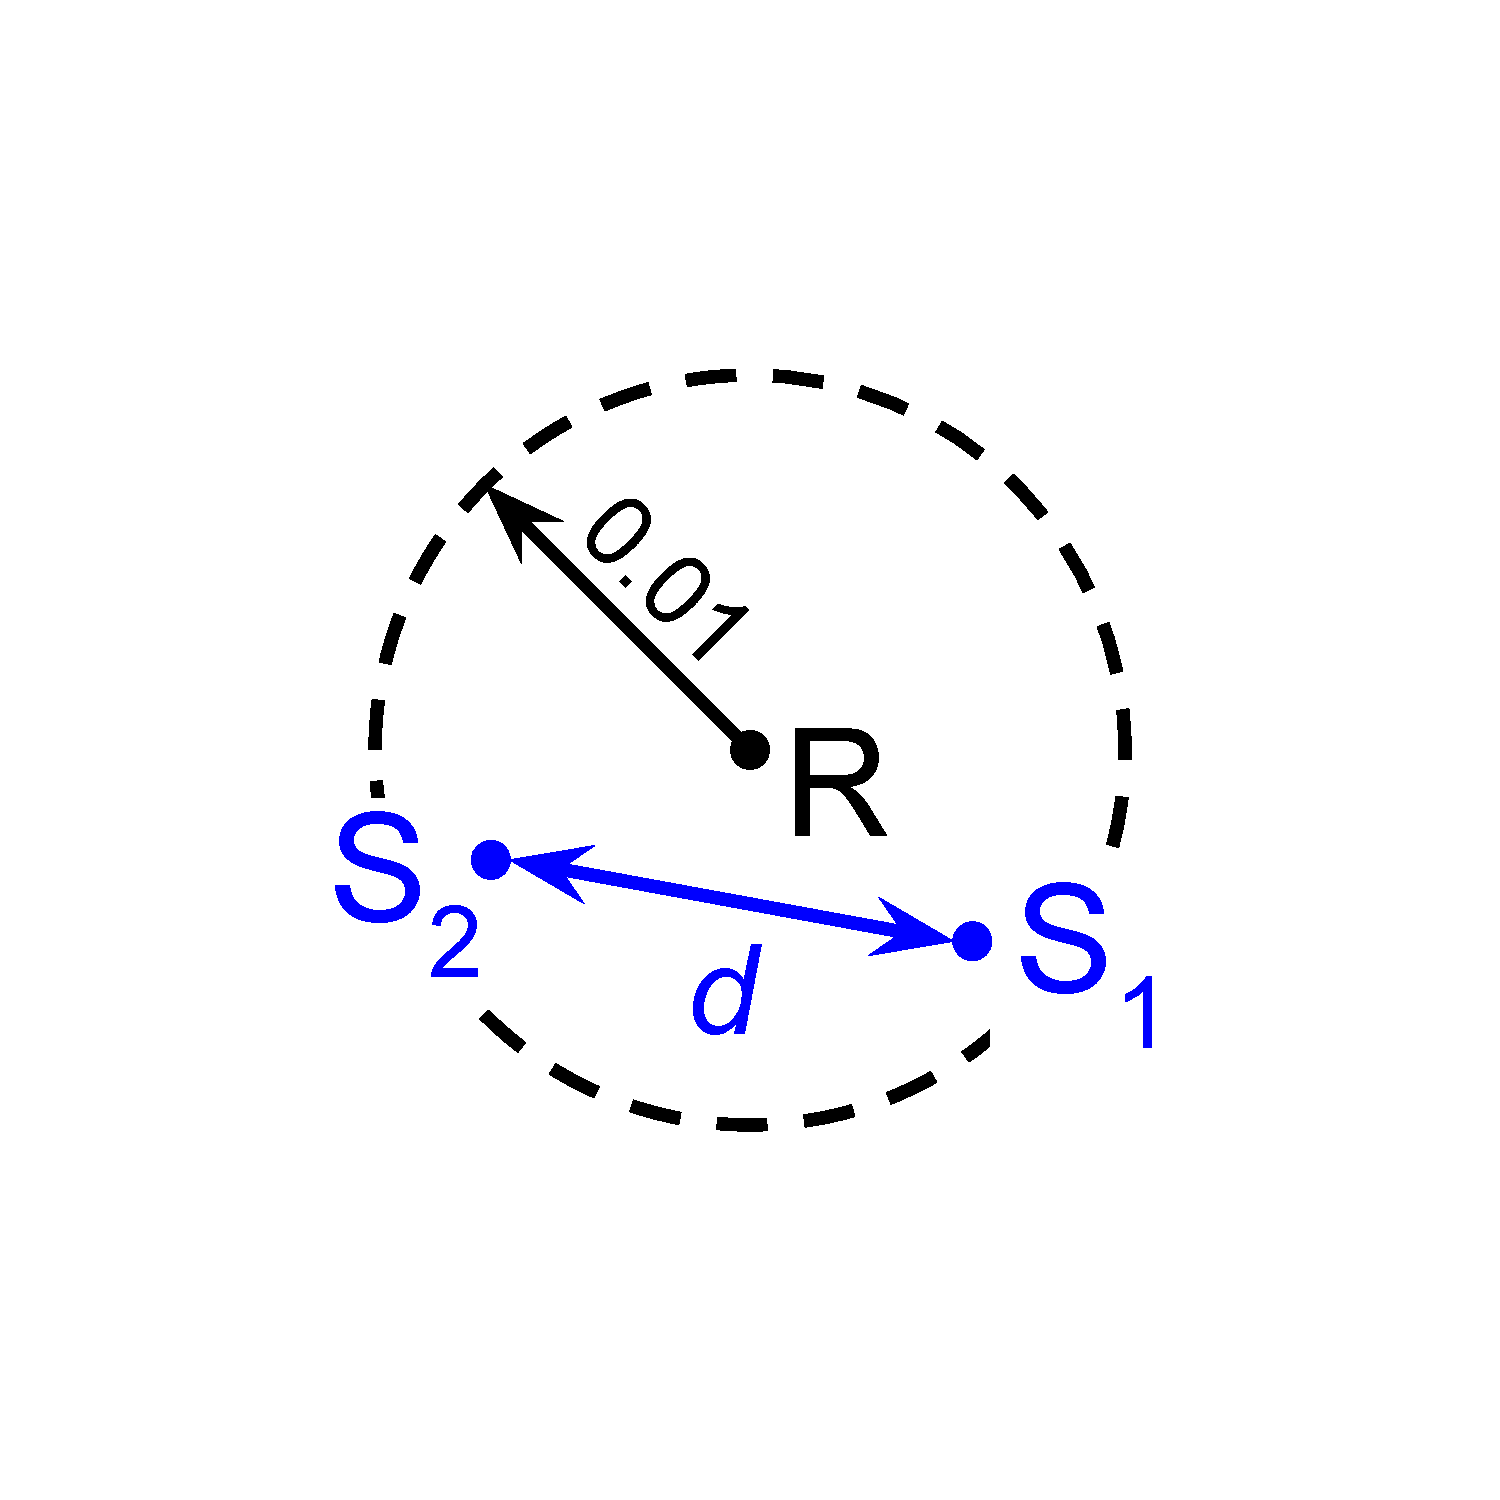
\includegraphics[width=0.5\linewidth,trim=5cm 5cm 5cm 5cm, clip]{img/dimensionality-statistic}
\end{center}
\end{minipage}%
\begin{minipage}{0.5\textwidth}
\caption{
Sampling process used to measure similarity constraint.
First, a constraining tag $R$ was randomly sampled.
Then, tags were randomly drawn until two tags $S_1$ and $S_2$ with distance to $R$ less than 0.01 were obtained.
Finally, similarity constraint was measured as the distance $d$ between $S_1$ and $S_2$.
}
\label{fig:dimensionality_measure}
\end{minipage}
\end{subfigure}
\end{minipage}
\begin{subfigure}[b]{\linewidth}
\begin{minipage}{0.6\linewidth}
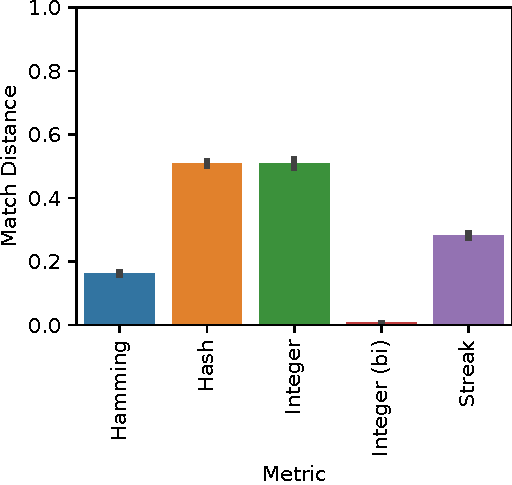
\includegraphics[width=\linewidth]{img/sphere/bitweight=0dot5+seed=1+title=dimensionality_barplot+_data_hathash_hash=c0f6c5cf854ff253+_script_fullcat_hash=03ce1e318a24a109+ext=}
\end{minipage}
\begin{minipage}{0.35\linewidth}
\caption{
Mean similarity constraint.
Error bars represent 95\% confidence intervals.
}
\label{fig:sphere_barplot}
\end{minipage}
\end{subfigure}
\begin{minipage}{\linewidth}
\begin{subfigure}[b]{\linewidth}
\centering
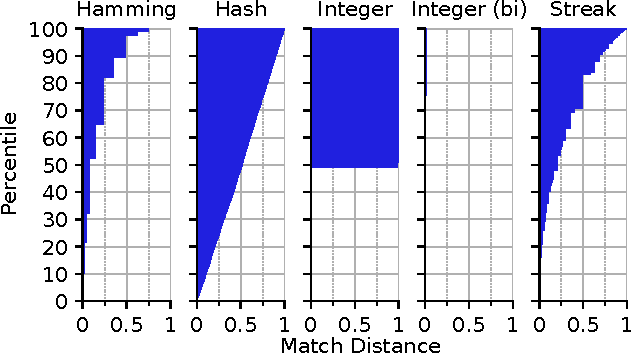
\includegraphics[width=\linewidth]{img/sphere/bitweight=0dot5+seed=1+title=dimensionality_distnplot+_data_hathash_hash=c0f6c5cf854ff253+_script_fullcat_hash=bea2a31376bf6bd0+ext=}
\begin{minipage}{0.8\textwidth}
\caption{
Distributions of sampled similarity constraint values.
Each visualization arranges individually sampled observations (thin horizontal bars) vertically in descending order.
The $y$ axis can be interpreted as ranging form the \nth{0} percentile of outcomes (bottom) to \nth{100} percentile (top) with horizontal bar width showing similarity constraint at a certain percentile.
}
\label{fig:sphere_distnplot}
\end{minipage}
\end{subfigure}
\end{minipage}

\caption{
Similarity constraint of tag-matching metrics.
Figure \ref{fig:dimensionality_measure} summarizes the sampling process used to measure similarity constraint.
Figures \ref{fig:sphere_barplot} and \ref{fig:sphere_distnplot} compare distributions of similarity constraint across metrics.
}
\label{fig:sphere}

\end{center}
\end{figure*}


To characterize similarity constraint for a metric $m$, we randomly sampled 5,000 target tags.
Then, for each target tag $R$ we randomly sampled tags until we found two secondarily-sampled tags $S_1$ and $S_2$ that were within a 0.01 match distance radius from the target.
That is, we chose $S_1$ and $S_2$ such that $m(R, S_1) < 0.01$ and $m(R, S_2) < 0.01$.
Finally, we computed the match distance $d = m(S_1, S_2)$ between the pair of secondarily-sampled tags.
Figure \ref{fig:dimensionality_measure} summarizes this process.

Figure \ref{fig:sphere_barplot} provides our estimate of the similarity constraint statistic for each metric, with error bars representing a 95\% confidence interval.
Figure \ref{fig:sphere_distnplot} shows the distribution of the similarity constraint statistic values among the 5,000 replicate samples in greater detail.

In a Euclidean space, similarity constraint corresponds to the average distance between points uniformly sampled from inside a ball (\textit{e.g.}, in two dimensions a circle, in three dimensions a sphere, \textit{etc.}).
In Euclidean space, this average distance increases with dimensionality.
For reference, in a one-dimensional Euclidean space similarity constraint would measure approximately 0.0067.
In a two dimensional Euclidean space, it would measure approximately  0.0091.
In 32 dimensions, it would measure 0.0137 \citep{dunbar1997average}.
So, in some sense, this similarity constraint metric can be interpreted as an indirect measure of dimensionality.
However, as we'll see in Section \ref{sec:detour_difference}, the Hamming, hash, and streak metric impose a decidedly non-Euclidean geometry.

\subsubsection{Hash Metric}

The hash metric exhibits a very loose similarity constraint of 0.5083 in the mean case.
Secondarily-sampled match distances are uniformly distributed between 0 and 1.
This is unsurprising:
given any particular set of operands, a well-behaved hash function should yield a uniform distribution of hash results.
As expected, the hash metric exhibits no geometric structure.

\subsubsection{Hamming Metric}

The Hamming metric exhibits a tighter range of sampled similarity constraint values.
We estimated mean similarity constraint as 0.1627.
As shown in Figure \ref{fig:sphere_distnplot}, many secondarily-sampled tag pairs are biased towards low match distances.
However, secondarily-sampled tag pairs that break this constraint are also not uncommon.
Among our 5,000 trials, we observed distances between secondarily-sampled tags as high as 0.7499.

Why is our estimate of the Hamming metric similarity constraint so much higher than the expected value of 0.0137 in a 32-dimensional Euclidean space?
This phenomenon appears to be due to the uniformification process we applied to map raw match distances to a uniform distribution.
We also calculated this statistic for the raw Hamming metric without uniformification, increasing the radius of our sampling ball to 0.25.
(Only the exact target 32-bit tag itself falls within a sampling radius of 0.01.)
The \textit{a priori} expected distance between sampled points within a 32-dimensional ball with radius 0.25 is 0.3415.
Our estimate of similarity constraint for the raw Hamming metric falls nearly in line with expectation at 0.3312.

\subsubsection{Streak Metric}

The streak metric exhibited the second-loosest similarity constraint statistic with a mean value sampled at 0.2813.
For this metric, we observed distances between secondarily-sampled tags as high as 0.9993.
The streak metric retains some geometric constraint in the mean case, but allows for outliers that strongly break similarity constraint.

\subsubsection{Integer Metric}

The integer metric exhibits loose similarity constraint in the mean case.
We estimated this value as 0.5092.
However, this looser mean similarity constraint appears to be an artifact of averaging between two very tight constraints: a tight constraint to 0 in one case and a tight constraint to 1 in the other.
Figure \ref{fig:sphere_distnplot} confirms that all sampled match distances fall under one of these cases.
Because of the asymmetrical definition of the integer metric, half of pairs of similar scalar values will be in ascending order (resulting in a match distance close to 0) and half will be in descending order (resulting in wraparound search and a match distance close to 1).
The integer metric appears to allow for a pair of tags closely related to a third tag either very strongly match or very weakly match, but permits no intermediate outcomes.

\subsubsection{Bidirectional Integer Metric}

For the bidirectional integer metric, we measured the similarity constraint statistic as 0.0068.
This falls in line with expectation: this metric is essentially identical to a one-dimensional Euclidean space.
As shown in Figure \ref{fig:sphere_distnplot}, the secondarily-sampled match distances are entirely bounded by the diameter of 0.02.
This metric not only exhibits tight similarity constraint in the mean case, but also permits no outlying similarity constraint outcomes.

\subsection{Dissimilarity Constraint} \label{sec:dissimilarityconstraint}

\begin{figure}
\begin{center}

\begin{subfigure}[b]{\columnwidth}
\centering
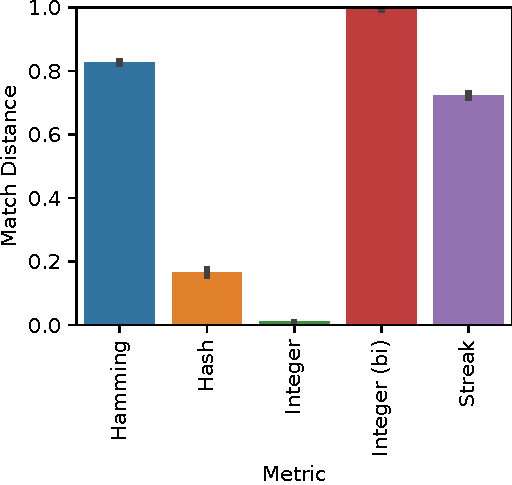
\includegraphics[width=\columnwidth]{{{sphere_reverse/bitweight=0.5+seed=1+title=dimensionality_barplot+_data_hathash_hash=7eaa832497d2f3cb+_script_fullcat_hash=03ce1e318a24a109+ext=}}}
\caption{
TODO
}
\label{fig:sphere_reverse_distnplot}
\end{subfigure}


\begin{subfigure}[b]{\columnwidth}
\centering
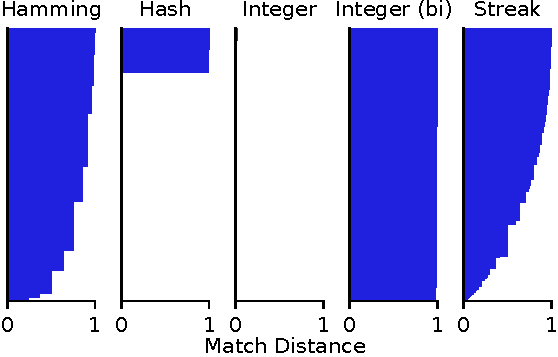
\includegraphics[width=\columnwidth]{{{sphere_reverse/bitweight=0.5+seed=1+title=dimensionality_distnplot+_data_hathash_hash=7eaa832497d2f3cb+_script_fullcat_hash=03ce1e318a24a109+ext=}}}
\caption{
TODO
}
\label{fig:sphere_reverse_barplot}
\end{subfigure}

\caption{
TODO
}
\label{fig:sphere_reverse}

\end{center}
\end{figure}

% \begin{figure}
\begin{center}

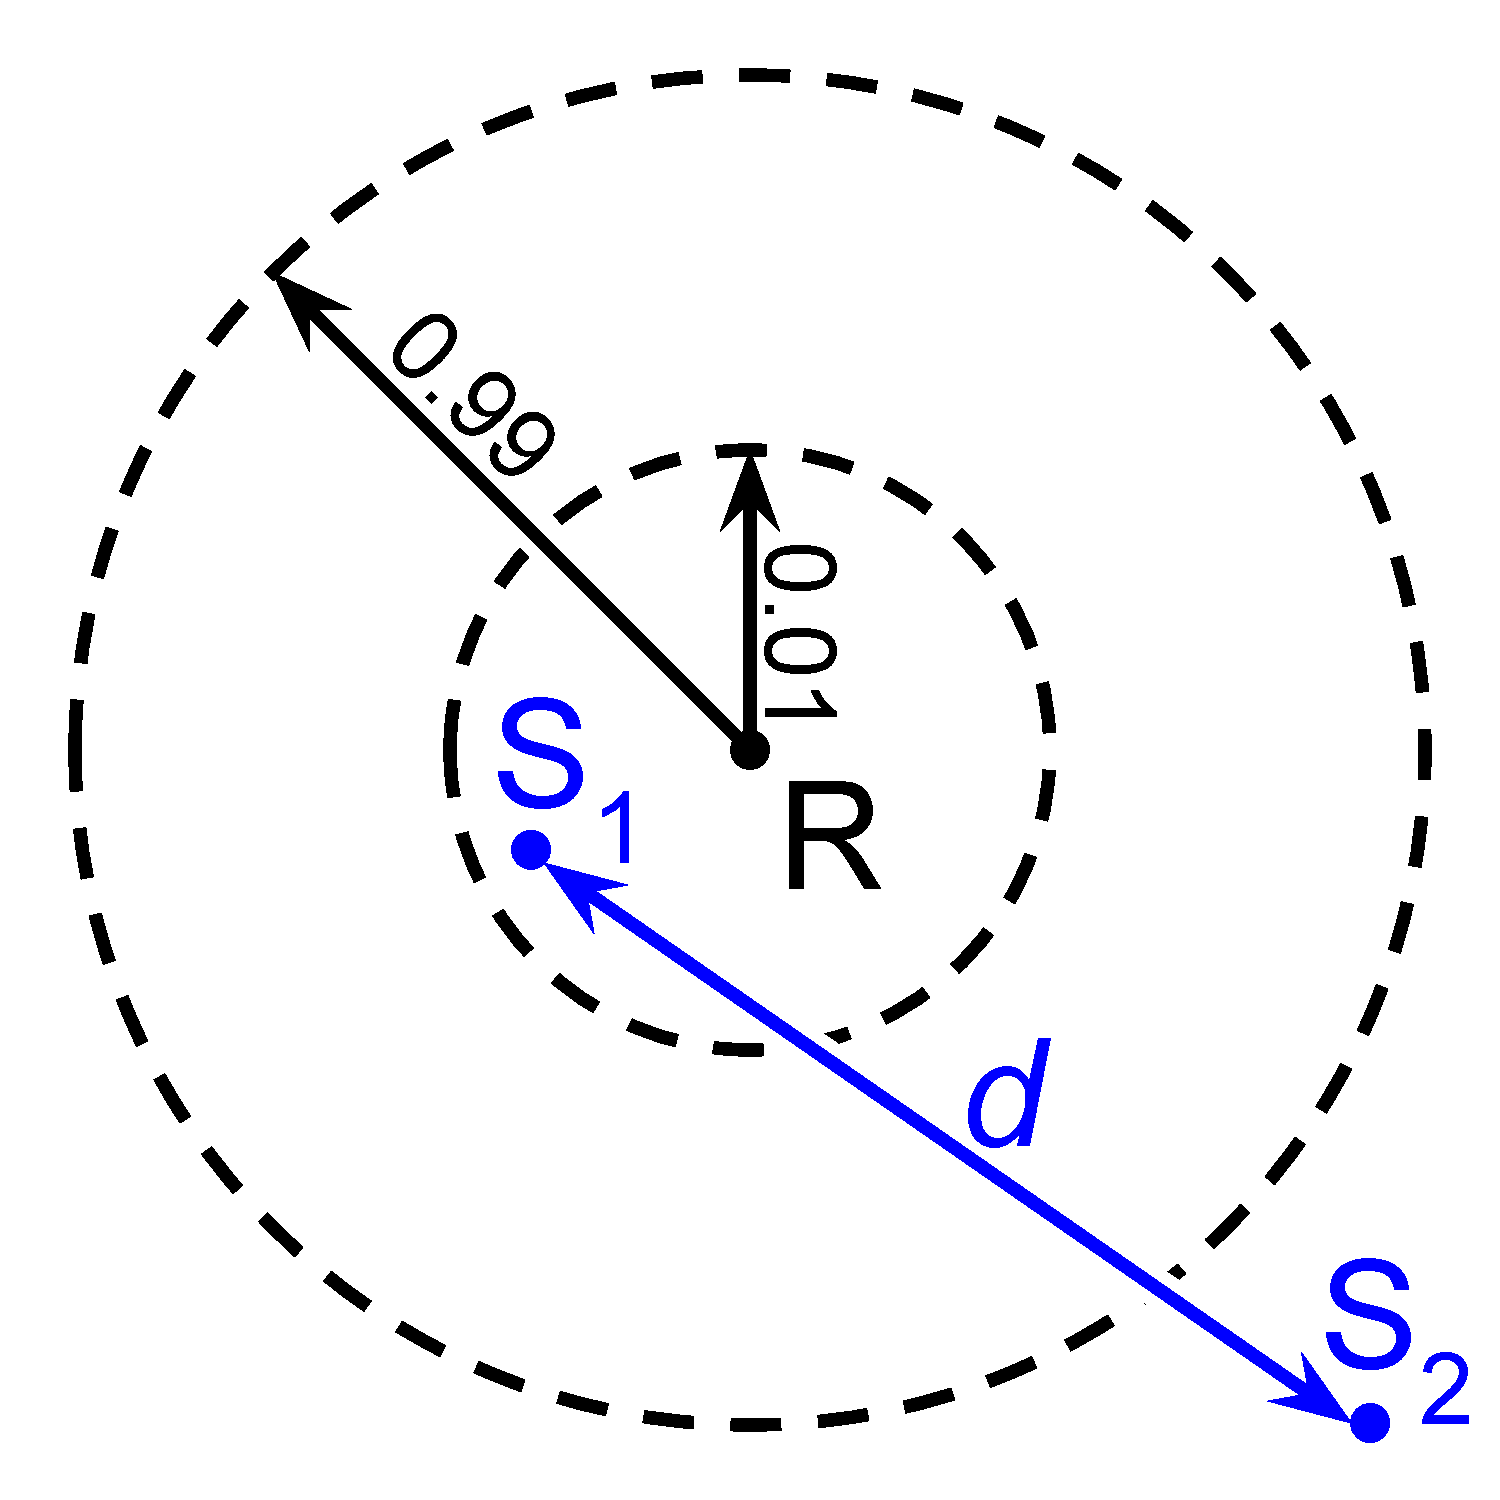
\includegraphics[width=0.5\linewidth]{elasticity-statistic}
\caption{
Dissimilarity statistic
}

\caption{
A schematic depicting the process used to generate the dissimilarity statistic for each metric.
}
\label{fig:dissimilarity_statistic}

\end{center}
\end{figure}


To characterize dissimilarity constraint for each metric $m$, we randomly sampled 5,000 target tags.
Then, for each target tag $R$ we randomly sampled tags until we found a secondarily-sampled tag $S_1$ that was within a 0.01 match distance radius from $R$ and a secondarily-sampled tag $S_2$ that was outside a 0.99 match distance radius from the $R$.
That is, we chose $S_1$ and $S_2$ such that $m(R, S_1) < 0.01$ and $m(R, S_2) > 0.99$.
Finally, we computed the match distance between $S_2$ and $S_1$, $d = m(S_2, S_1)$.
Figure \ref{fig:dissimilarity_statistic} summarizes this process.

Figure \ref{fig:sphere_barplot} provides our estimate of the dissimilarity constraint statistic for each metric, with error bars representing a 95\% confidence interval.
Figure \ref{fig:sphere_distnplot} shows the distribution of the dissimilarity constraint statistic values among the 5,000 replicate samples in greater detail.

These results tell a similar story to our similarity constraint findings.

\subsubsection{Hash Metric}
The hash metric exhibited no geometric structure --- $S_1$ and $S_2$ were uniformly likely to exhibit any match distance between 0 and 1.

\subsubsection{Hamming Metric}

The Hamming metric exhibited stronger geometric structure in the mean case than the streak metric.
Mean secondarily-sampled distance was 0.8248.
The Hamming metric also exhibited less extreme tail-end outcomes than the streak metric.
We observed match distances between the secondarily-sampled tags only as low as 0.2355.

\subsubsection{Streak Metric}

The streak metric exhibited some geometric structure in the mean case.
We observed a mean secondarily-sampled distance 0.7127, significantly greater than the mean distance of 0.5 expected between arbitrarily-sampled tags.

However, outcomes that strongly broke geometric constraints also occurred.
We observed distances between secondarily-sampled tags as low as 0.0002.

\subsubsection{Integer Metric}

Again, the unidirectional integer metric exhibited a quirky result due to its noncommutative nature.
The mean distance between secondarily-sampled tags was 0.0100.
That is, instead of observing poor matches as we would expect, secondarily-sampled tags were much closer together than expected under arbitrary sampling.
As shown in Figure \ref{fig:sphere_distnplot}, \textit{all} secondarily-sampled distances observed with this metric were extremely small.
So, although in the opposite way from what we would expect, match distances were still tightly constrained.

The mechanism behind this result stems from the metric's asymmetrical nature.
Under this metric, if you sample a tag that is close to a target it will be numerically slightly larger than the target.
Likewise, if you sample a tag that is very far from a target, it will be numerically slightly smaller than the target (due to wraparound).
Then, explaining this counterintuitive result, the distance from the slightly smaller to the slightly larger tag will be small.

\subsubsection{Bidirectional Integer Metric}

The bidirectional integer metric was highly constrained in both the mean and tail-end cases.
The smallest distance between secondarily-sampled tags observed was 0.9802.

\subsection{Detour Difference} \label{sec:detour_difference}

\begin{figure}
\begin{center}

\begin{minipage}{\linewidth}
\begin{subfigure}[b]{\linewidth}
\begin{minipage}{0.5\textwidth}
\begin{center}
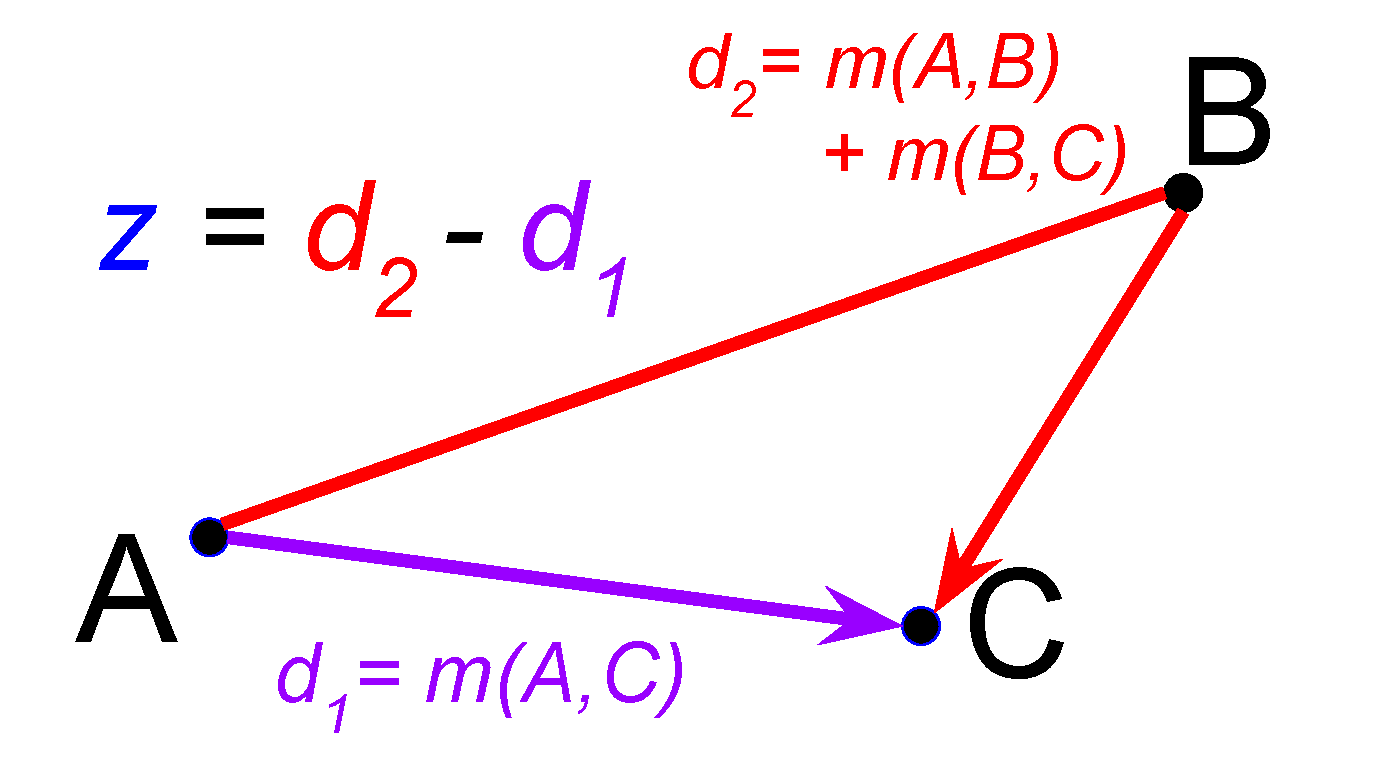
\includegraphics[width=\linewidth,trim=2cm 5cm 2cm 5cm, clip]{detour-difference}
\end{center}
\end{minipage}%
\begin{minipage}{0.5\textwidth}
\caption{
Sampling process used to evaluate detour difference, $z$.
} \label{fig:detour_difference_cartoon}
\end{minipage}
\end{subfigure}
\end{minipage}

\begin{minipage}{\linewidth}
\begin{subfigure}[b]{\linewidth}
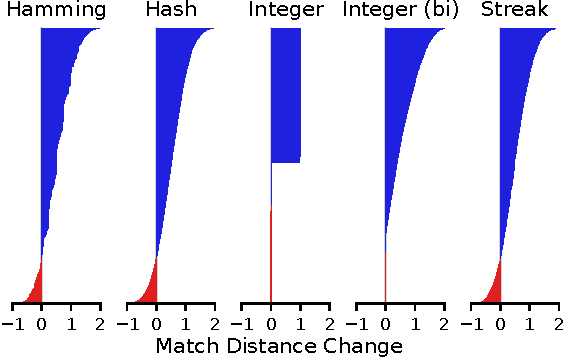
\includegraphics[width=\linewidth]{detour_difference/bitweight=0dot5+seed=1+title=low-triplet-analysis+_data_hathash_hash=6b0749ef97a58721+_script_fullcat_hash=297c4fe09078e17b+ext=}
\caption{
Distributions of detour distance difference for triplets of randomly sampled tags.
Each bar sliver represents an independently sampled observation.
A positive value (colored blue) indicates that total distance increased with the addition of an intermediate stop.
A value of exactly 0 indicates an intermediate stop had no effect on total distance.
A negative value (colored red) indicates violation of the triangle inequality: taking an intermediate stop reduced the total distance travelled.
} \label{fig:detour_difference_distribution}

\end{subfigure}
\end{minipage}

\caption{
Detour difference of tag-matching metrics.
}
\label{fig:detour_difference}

\end{center}
\end{figure}


Similarity constraint and dissimilarity constraint quantify the geometric constraint imposed under preexisting strong matches and strong mismatches, respectively.
To complement these measures, we set out to characterize the regularity, in a loose sense, of each space more broadly.
This led us to our ``detour difference'' measure, which quantifies tag matching spaces' respect for the triangle inequality.

Intuitively, detour difference is a measure of how adding a randomly-chosen waypoint affects total distance between pre-existing start and end points.
Under the triangle inequality, the direct route is always shortest.
So, if the triangle inequality is respected, detour difference should always be non-negative.

To measure detour difference, we uniformly sampled 5,000 triplets of tags $A$, $B$, and $C$.
Then, for each metric $m$ we calculated the $m(A, B) + m(B, C) - m(A, C)$.
Figure \ref{fig:detour_difference_cartoon} provides a schematic of this process.

Figure \ref{fig:detour_difference_distribution} plots the distribution of the detour difference statistic for each metric.
The Hamming, hash, and streak metrics show evidence of ``shortcuts'' that violate the triangle inequality.%
\footnote{%
The raw Hamming metric does respect the triangle inequality, so presumably this result is due to the uniformification.
}
For the Hamming, streak, and hash metrics the most extreme shortening detours observed were -0.76, -0.91, and -0.94, respectively.
The integer and bidirectional integer metrics only exhibited shortening detours up to -0.02, which were due to minor stochastic imperfections of the uniformification process.
As would be expected given their Euclidean basis, shortening detours were otherwise nonexistent for the integer metrics.

Surprisingly, given divergent results from the similarity and dissimilarity constraint measures, the distributions of detour difference for these three metrics appear similar.
This suggests that geometric differences between these metrics are specially accentuated in contexts of preexisting strong matching and mismatching constraint.
